\documentclass[12pt]{article}

\usepackage{sbc-template}
\usepackage{graphicx,url}
\usepackage[T1]{fontenc}
\usepackage[utf8]{inputenc}
\usepackage[brazil]{babel}
\usepackage{enumitem}
\usepackage{placeins}

% Defina aqui a hifenização de palavras que o LaTeX quebra errado
% (ex.: \hyphenation{com-pu-ta-ção al-go-rit-mo})

\sloppy

\title{Maximização da Taxa de Transferência Usando \textit{Sockets} TCP:\\ Avaliação de um Servidor de Chat com Múltiplos Clientes}

\author{
	Breno Cerqueira Reis Nakamura (168765),
	Estevan Teixeira Santos (168826),
	\\Vinícius Augusto Landim Andrade (169251)
}

\address{
}

\renewcommand{\instnum}{}

\begin{document}

\maketitle
\vspace{-1cm}
\begin{resumo}
  Este trabalho avalia a capacidade máxima de transmissão de dados de clientes
  para um servidor em uma aplicação de chat baseada em \textit{sockets} TCP.
  Para isso, modificaram-se o cliente e o servidor originais, de modo que o
  cliente transmita dados continuamente durante um intervalo definido e o
  servidor contabilize os bytes recebidos em cada conexão. Realizaram-se
  experimentos com 1 a 10 clientes simultâneos em três cenários, sendo eles
  \textit{loopback}, rede local cabeada e rede sem fio. Na rede cabeada, a taxa
  agregada cresceu até saturar em cerca de 941~Mbps, limite do enlace Gigabit
  Ethernet, enquanto no Wi-Fi permaneceu entre 60 e 90~Mbps, independentemente
  do número de clientes. Já no \textit{loopback}, a taxa atingiu 180~Gbps com
  cinco clientes e diminuiu a partir daí devido à disputa pelo processador.
\end{resumo}


\section{Introdução}

A taxa de transferência efetiva de uma aplicação em rede depende não apenas da
capacidade do enlace físico, mas também da forma como a aplicação utiliza os
recursos oferecidos pelo sistema operacional. Nesse contexto, este trabalho tem
como objetivo avaliar a capacidade máxima de transmissão de dados dos clientes
para o servidor em uma aplicação de chat baseada em \textit{sockets} TCP,
medindo a taxa de transmissão agregada recebida pelo servidor à medida que o
número de clientes simultâneos varia de 1 a 10.

A aplicação original é composta por dois programas, \texttt{chat\_server} e
\texttt{chat\_client}. O servidor aceita conexões em uma porta TCP e cria uma
\textit{thread} para cada cliente conectado, de modo que vários usuários possam
conversar ao mesmo tempo. Cada \textit{thread} lê as mensagens do seu cliente
byte a byte até encontrar o caractere de nova linha e, em seguida, repassa a
mensagem a todos os demais clientes conectados. Já o cliente funciona de forma
interativa, pois utiliza uma \textit{thread} para ler o texto digitado pelo
usuário e enviá-lo ao servidor e outra para receber e exibir as mensagens dos
demais participantes.

Embora adequado para uma conversa entre usuários, esse funcionamento não permite
medir a capacidade de transmissão da conexão. Em primeiro lugar, o envio de
dados depende da digitação manual, o que torna o volume transmitido pequeno e
irregular. Além disso, a leitura byte a byte exige uma chamada ao sistema
operacional para cada caractere recebido, e o repasse das mensagens a todos os
clientes, protegido por um único \textit{mutex} global, multiplica o tráfego e
serializa o trabalho das \textit{threads}. Por fim, a aplicação não registra a
quantidade de dados recebidos nem o tempo de transmissão, de forma que não há
como calcular a taxa alcançada.

Diante disso, os códigos foram modificados para que o cliente transmita dados
continuamente durante um intervalo de tempo definido, sem intervenção do
usuário, e para que o servidor contabilize os bytes efetivamente recebidos em
cada conexão e calcule a taxa de transmissão agregada. Com essas alterações,
foram realizados experimentos com 1 a 10 clientes simultâneos em três cenários,
sendo eles a comunicação local na própria máquina (\textit{loopback}), uma rede
local cabeada e uma rede local sem fio. Assim, busca-se compreender como o
aumento do número de clientes afeta a capacidade de transmissão do servidor e
identificar quais fatores limitam o desempenho em cada cenário.

\section{Desenvolvimento}\label{sec:desenvolvimento}

As modificações preservaram a base da aplicação original, isto é, a comunicação
por \textit{sockets} TCP, o uso de uma \textit{thread} por conexão no servidor e
o envio inicial do nome de cada cliente terminado por nova linha. Por outro
lado, as partes voltadas à interação com o usuário foram substituídas por
mecanismos de geração de carga, de sincronização e de medição. O código-fonte
modificado está disponível no repositório
\url{https://github.com/brenonak/tcp-throughput-chat/}.

\subsection{Cliente}

O novo cliente deixou de ser interativo e passou a funcionar como um gerador de
carga. Ao ser executado, ele recebe o endereço do servidor, a porta, a duração
da transmissão e a quantidade $N$ de conexões desejadas, e então cria $N$
\textit{threads}, cada uma responsável por uma conexão TCP própria. Dessa forma,
um único programa é capaz de simular vários clientes simultâneos, pois, do ponto
de vista do servidor, cada conexão é independente, com seu próprio
\textit{socket}, seu próprio estabelecimento de conexão e sua própria
\textit{thread} de atendimento. Essa escolha dispensa o uso de dez computadores
ou de dez processos separados e, além disso, facilita a sincronização do início
dos testes.

Após estabelecer a conexão, cada \textit{thread} envia um nome de identificação,
mantendo o protocolo do chat original, e aguarda uma mensagem de início enviada
pelo servidor. Somente após recebê-la a \textit{thread} começa a transmitir,
enviando repetidamente um bloco de 64~KiB até que o tempo definido se esgote, o
que é verificado por um relógio monotônico do sistema. Ao final, a
\textit{thread} encerra a conexão. Como o conteúdo dos dados não importa para a
medição, o bloco é preenchido uma única vez antes do envio, o que evita qualquer
processamento adicional durante a transmissão e faz com que o cliente se dedique
exclusivamente a enviar dados.

\subsection{Servidor}

O servidor passou a aguardar exatamente $N$ conexões, criando uma
\textit{thread} para cada uma, assim como na versão original. Cada
\textit{thread} lê o nome do seu cliente e registra a conexão e, em seguida,
todas aguardam em uma barreira de sincronização. Quando todas as conexões estão
registradas, o servidor marca o instante inicial da medição e envia a mensagem
de início a todos os clientes. Com isso, nenhuma conexão começa a transmitir
antes de as demais estarem prontas, e todas as medições usam um único relógio, o
do servidor, o que dispensa a sincronização dos relógios entre máquinas
diferentes.

Durante a transmissão, cada \textit{thread} lê os dados em blocos de 64~KiB,
descarta o conteúdo e soma a quantidade de bytes recebidos a um contador
exclusivo da sua conexão. Diferentemente do servidor original, não há leitura
byte a byte, repasse de mensagens aos demais clientes nem impressão na tela, e o
contador é atualizado por uma operação atômica, sem uso de \textit{mutex}.
Assim, as \textit{threads} trabalham de forma independente e o servidor realiza
apenas o trabalho essencial de receber os dados, o que permite avaliar o limite
da transmissão em vez do custo da própria aplicação.

Paralelamente, uma \textit{thread} amostradora registra a cada segundo o total
acumulado de cada conexão, junto com o instante exato da leitura. Essas amostras
permitem calcular a taxa em um intervalo no qual a transmissão já está estável,
descartando o início e o fim de cada teste, como detalhado na
Seção~\ref{sec:metodologia}. Quando todos os clientes encerram suas conexões, o
servidor calcula a taxa de transmissão agregada e grava os resultados em
arquivos CSV. Caso alguma conexão apresente erro, o servidor encerra a execução
com falha, de modo que testes incompletos não sejam confundidos com resultados
válidos.

\subsection{Automação dos experimentos}

Além dos dois programas, desenvolveram-se \textit{scripts} para automatizar a
execução e a análise dos testes. Um executor inicia o servidor e os clientes
para cada quantidade de conexões e cada repetição, valida os resultados de cada
rodada a partir das amostras e registra também o uso do processador e o tráfego
de rede durante os testes. Em seguida, um \textit{script} de análise reúne as
rodadas válidas e gera as estatísticas e os gráficos apresentados na
Seção~\ref{sec:resultados}. Por fim, um conjunto de testes automatizados
verifica o protocolo de início, a validação das rodadas e a análise.

\section{Metodologia} \label{sec:metodologia}
\subsection{Ambiente experimental}

Os experimentos foram realizados em dois computadores, identificados como
D15-126 e ANVS14, cujas características estão resumidas na
Tabela~\ref{tab:ambiente}. Em ambos, os programas foram executados no Ubuntu
26.04 por meio do WSL2 (\textit{Windows Subsystem for Linux}), que executa o
Linux em uma máquina virtual leve dentro do Windows. Por esse motivo, a memória
indicada corresponde à parcela disponibilizada ao WSL, e não à memória total de
cada computador.

\begin{table}[ht]
\centering
\caption{Características das máquinas utilizadas.}
\label{tab:ambiente}
\begin{tabular}{lll}
\hline
 & \textbf{D15-126 (servidor)} & \textbf{ANVS14 (cliente)} \\
\hline
Processador & Intel Core i5-12500H & Intel Core Ultra 7 256V \\
Núcleos / \textit{threads} & 12 / 16 & 8 / 8 \\
Memória disponível no WSL & 7,6 GiB & 7,5 GiB \\
Sistema operacional & Ubuntu 26.04 (WSL2) & Ubuntu 26.04.1 (WSL2) \\
Versão do kernel & 6.18.33 & 6.6.87 \\
Compilador & gcc 15.2.0 & gcc 15.2.0 \\
Controle de congestionamento TCP & CUBIC & CUBIC \\
\hline
\end{tabular}
\end{table}

Foram avaliados três cenários de comunicação. No cenário de \textit{loopback},
cliente e servidor foram executados no mesmo computador (D15-126), de modo que
os dados não passam por nenhuma placa de rede e o desempenho depende apenas do
processador, da memória e da pilha TCP do sistema operacional. Já nos dois
cenários de rede local, o servidor foi executado no D15-126 e todas as conexões
partiram do ANVS14. Na rede cabeada, as máquinas foram ligadas por Ethernet
Gigabit, com enlace de 1~Gbps, na mesma sub-rede e sem roteador intermediário,
enquanto na rede sem fio a comunicação ocorreu por Wi-Fi.
% TODO: indicar qual máquina estava no Wi-Fi e o tipo de rede (ex.: roteador doméstico).

Nos cenários de rede local, o tráfego também passou pelo encaminhamento entre o
Windows e o WSL, já que o WSL2 operava em modo NAT, com uma interface virtual de
MTU igual a 1492 bytes. Essa camada adicional faz parte do ambiente e,
portanto, influencia os resultados, como discutido na
Seção~\ref{sec:resultados}.

\subsection{Procedimento experimental}

Em cada cenário, executou-se uma campanha com 1 a 10 clientes simultâneos e
cinco repetições para cada quantidade, o que totaliza 50 rodadas por cenário e
150 rodadas no total. Em cada rodada, os clientes transmitiram continuamente
durante 30 segundos, enviando blocos de 64~KiB. Além disso, as rodadas foram
executadas em ordem crescente de clientes, com um intervalo de 5 segundos entre
elas para que as conexões anteriores fossem completamente encerradas.

Para garantir a comparabilidade dos resultados, todas as rodadas utilizaram o
mesmo código, compilado com as mesmas opções, e os mesmos parâmetros de
duração, tamanho de bloco e janela de medição. Ademais, o início sincronizado
pela mensagem de início garante que todas as conexões transmitam ao mesmo
tempo, enquanto o uso exclusivo do relógio do servidor evita erros causados
pela diferença entre os relógios das máquinas. Cada rodada também foi validada
automaticamente, com a verificação da consistência entre as amostras e o
resultado final, e as características do ambiente foram registradas no início
de cada campanha. Ao final, todas as 150 rodadas foram consideradas válidas.

\subsection{Cálculo da taxa de transmissão agregada}

A taxa agregada corresponde à soma das taxas de todas as conexões atendidas
pelo servidor. Como cada \textit{thread} mantém um contador próprio de bytes
recebidos, a \textit{thread} amostradora registra a cada segundo o valor
acumulado de cada conexão. Dessa forma, a quantidade de dados recebida em um
intervalo é obtida pela diferença entre os contadores no início e no fim desse
intervalo, somada para todas as conexões, e a taxa agregada é dada por
\begin{equation}
R = \frac{8 \sum_{i=1}^{N} \left[ B_i(t_f) - B_i(t_i) \right]}{(t_f - t_i) \times 10^6},
\end{equation}
em que $N$ é o número de clientes, $B_i(t)$ é o total de bytes recebidos pela
conexão $i$ até o instante $t$, e $t_i$ e $t_f$ são os instantes inicial e
final da janela de medição. O fator 8 converte bytes em bits, e a divisão por
$10^6$ expressa o resultado em Mbps.

Os primeiros e os últimos 5 segundos de cada rodada foram descartados, pois no
início o TCP ainda está aumentando sua taxa de envio e, no fim, as conexões são
encerradas em instantes ligeiramente diferentes. Assim, a janela de medição
corresponde a aproximadamente 20 segundos de transmissão estável, e os
instantes $t_i$ e $t_f$ são os valores reais registrados pelo relógio do
servidor, e não valores nominais. Além disso, apenas os dados da aplicação são
contabilizados, sem os cabeçalhos dos protocolos nem as mensagens de controle,
de modo que a taxa medida corresponde à vazão útil (\textit{goodput}).

Por fim, para cada quantidade de clientes, considerou-se como
\textit{throughput} agregado máximo o maior valor obtido entre as cinco
repetições, conforme solicitado no enunciado. Complementarmente, calcularam-se
a média, o desvio padrão e o intervalo de confiança de 95\% das repetições, que
indicam a estabilidade das medições.

\section{Resultados e Discussões}\label{sec:resultados}

A Tabela~\ref{tab:resultados} apresenta a taxa de transmissão agregada máxima e
média obtida em cada cenário para 1 a 10 clientes simultâneos, enquanto a
Figura~\ref{fig:maximo} mostra a taxa máxima em escala logarítmica, necessária
porque os cenários diferem em várias ordens de grandeza. De modo geral, o
comportamento observado dependeu menos do servidor e mais do recurso que
limitava a transmissão em cada cenário, isto é, o enlace físico na rede
cabeada, o meio sem fio no Wi-Fi e o processador no \textit{loopback}.

\begin{table}[ht]
\centering
\caption{Taxa de transmissão agregada máxima e média, em Mbps, por número de
clientes simultâneos ($N$).}
\label{tab:resultados}
\small
\begin{tabular}{crrrrrr}
\hline
 & \multicolumn{2}{c}{\textbf{Loopback}} & \multicolumn{2}{c}{\textbf{Rede cabeada}} & \multicolumn{2}{c}{\textbf{Wi-Fi}} \\
$N$ & Máx. & Média & Máx. & Média & Máx. & Média \\
\hline
1  & 50\,743  & 49\,375  & 209,5 & 202,9 & 83,5 & 61,2 \\
2  & 99\,014  & 96\,996  & 400,5 & 387,5 & 86,1 & 81,4 \\
3  & 152\,189 & 149\,316 & 778,0 & 743,6 & 89,7 & 68,0 \\
4  & 176\,058 & 171\,900 & 940,6 & 939,7 & 80,1 & 68,4 \\
5  & 180\,762 & 176\,294 & 941,3 & 940,9 & 70,4 & 65,0 \\
6  & 178\,625 & 166\,697 & 941,5 & 940,4 & 78,1 & 62,2 \\
7  & 165\,462 & 160\,222 & 941,1 & 941,1 & 86,9 & 68,7 \\
8  & 149\,552 & 147\,613 & 941,6 & 941,1 & 84,0 & 72,0 \\
9  & 145\,786 & 145\,057 & 941,2 & 941,0 & 91,6 & 77,1 \\
10 & 144\,104 & 143\,400 & 941,0 & 941,0 & 80,1 & 68,2 \\
\hline
\end{tabular}
\end{table}

\begin{figure}[ht]
\centering
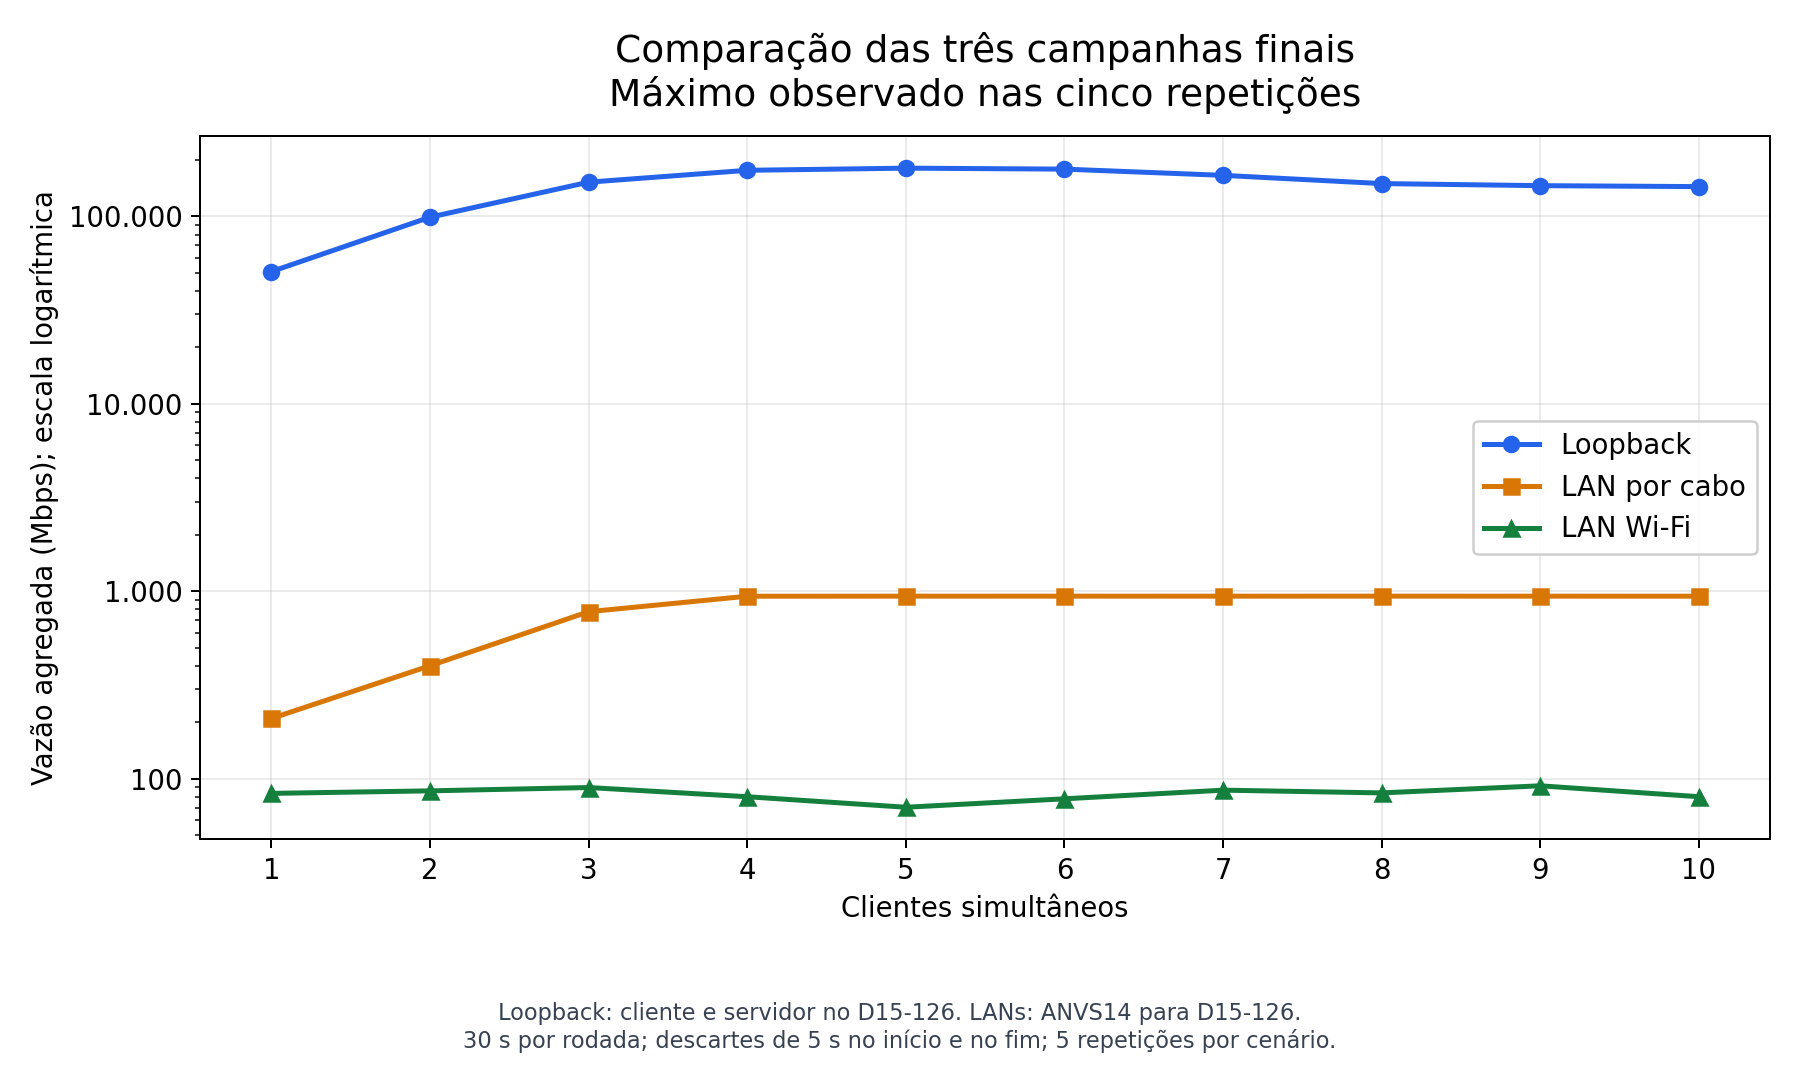
\includegraphics[width=\textwidth]{figs/comparacao_maximo_log.png}
\caption{Taxa de transmissão agregada máxima em função do número de clientes
nos três cenários, em escala logarítmica.}
\label{fig:maximo}
\end{figure}

\subsection{Rede cabeada}

Na rede cabeada, a taxa agregada cresceu de forma aproximadamente proporcional
ao número de clientes até três conexões, passando de cerca de 203~Mbps para
744~Mbps em média. A partir de quatro clientes, contudo, a taxa estabilizou em
torno de 941~Mbps, com variação inferior a 2~Mbps entre as repetições, como
mostra a Figura~\ref{fig:lan}. Esse valor coincide com o limite teórico de
vazão útil do TCP em um enlace Gigabit Ethernet. Isso ocorre porque, embora o
enlace transmita 1~Gbps, parte de cada quadro é ocupada pelos cabeçalhos
Ethernet, IP e TCP e pelo intervalo obrigatório entre quadros, de modo que, com
a MTU de 1492 bytes utilizada, apenas 1440 de cada 1530 bytes ocupados no meio
são dados da aplicação, o que corresponde a aproximadamente 941~Mbps.
Portanto, a partir de quatro clientes, o gargalo passou a ser o próprio enlace
físico.

\begin{figure}[ht]
\centering
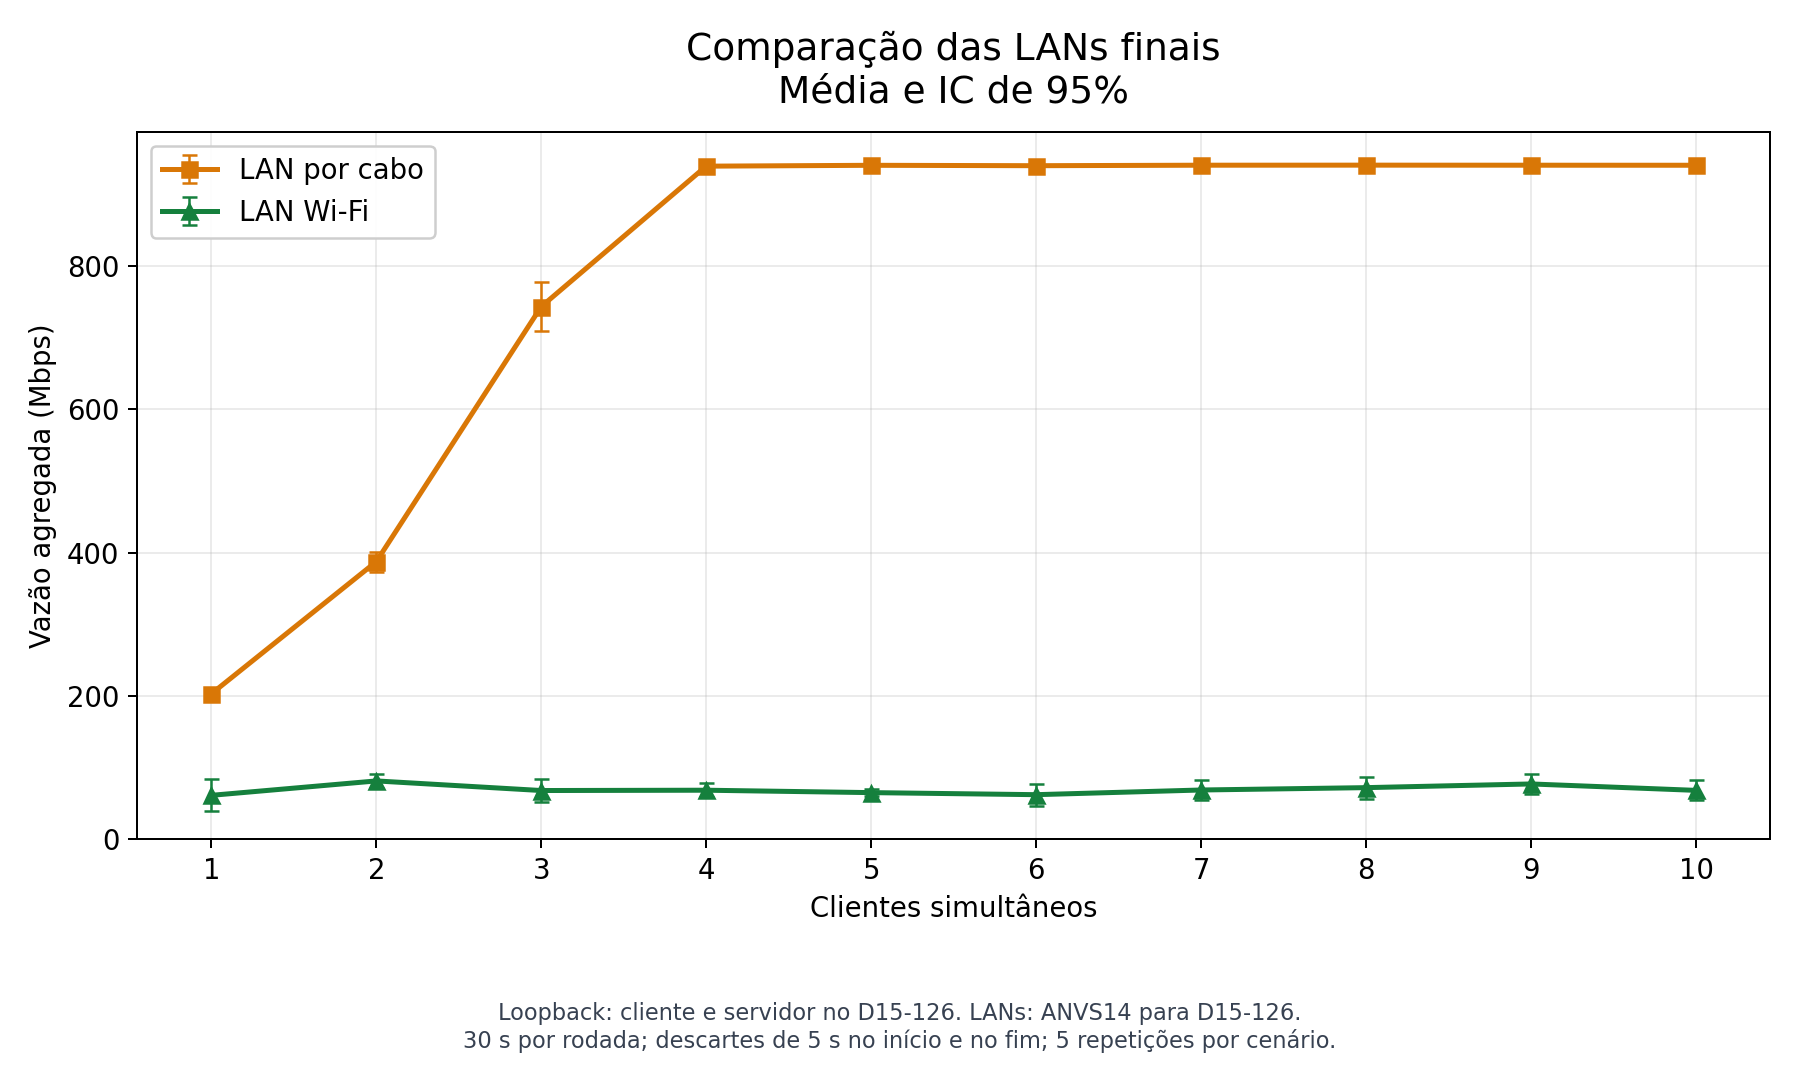
\includegraphics[width=.8\textwidth]{figs/comparacao_lan_media.png}
\caption{Taxa de transmissão agregada média nas redes cabeada e sem fio, com
intervalo de confiança de 95\%.}
\label{fig:lan}
\end{figure}

Por outro lado, com poucos clientes, cada conexão alcançou apenas cerca de 200
a 250~Mbps, bem abaixo da capacidade do enlace. Como os \textit{buffers} TCP
das máquinas são grandes em relação ao baixo atraso de uma rede local, é pouco
provável que esse limite se deva ao controle de fluxo do TCP. A explicação mais
provável é o encaminhamento entre o Windows e o WSL, que possivelmente processa
cada conexão de forma individual e impõe um limite de taxa por conexão. Dessa
forma, o aumento do número de clientes foi justamente o que permitiu somar as
taxas individuais até atingir a capacidade do enlace. Após a saturação,
entretanto, as conexões passaram a disputar a mesma banda e a divisão entre
elas tornou-se desigual, chegando a um caso em que a conexão mais lenta recebeu
cerca de um terço da taxa da mais rápida.

\subsection{Rede sem fio}

No cenário Wi-Fi, a taxa média permaneceu entre 61 e 81~Mbps para qualquer
número de clientes, e o maior valor observado foi de 91,6~Mbps, com nove
clientes. Diferentemente da rede cabeada, o aumento do número de conexões não
elevou a taxa agregada, pois o meio sem fio já era o gargalo desde o primeiro
cliente. Nesse tipo de rede, o canal é compartilhado, os dispositivos não
transmitem e recebem ao mesmo tempo, e a taxa efetiva depende da qualidade do
sinal, de interferências e de retransmissões, o que resulta em uma capacidade
bem inferior à nominal. Por esse motivo, os resultados também foram os mais
variáveis entre as repetições, como indicam os amplos intervalos de confiança
da Figura~\ref{fig:lan}, e a divisão da banda entre as conexões foi a mais
desigual entre os três cenários.

Observou-se ainda que, em parte das rodadas, a janela de medição se estendeu
por 21 a 26 segundos, em vez de 20. Isso ocorreu porque ainda havia dados em
trânsito quando os clientes pararam de enviar, o que atrasou o encerramento das
conexões. Embora isso não invalide as medições, a janela acabou incluindo parte
desse esvaziamento.

\subsection{Loopback}

No \textit{loopback}, os dados não atravessam nenhuma placa de rede, de modo
que a transmissão consiste basicamente em cópias de memória realizadas pelo
sistema operacional, primeiro do cliente para o espaço do sistema e, depois,
deste para o servidor. Por isso, as taxas foram muito superiores às das redes
locais, chegando a 180,8~Gbps no máximo e a 176,3~Gbps em média com cinco
clientes. Até três clientes, a taxa cresceu de forma praticamente linear, com
cerca de 49~Gbps por conexão, o que indica que cada conexão dispunha de
recursos de processamento suficientes. A partir de quatro clientes, contudo, o
ganho diminuiu e, após cinco clientes, a taxa passou a cair, chegando a
143,4~Gbps com dez clientes.

Esse comportamento é explicado pela disputa pelo processador. Como cliente e
servidor executam na mesma máquina, cada conexão ocupa duas \textit{threads}
ativas, uma de envio e outra de recepção. Com cinco clientes, já há dez
\textit{threads} ativas, mais do que os quatro núcleos de desempenho do
processador, e, a partir de oito clientes, o número de \textit{threads} supera
os 16 processadores lógicos disponíveis. Assim, as \textit{threads} passam a
compartilhar núcleos, a utilizar os núcleos de eficiência, mais lentos, e a ser
alternadas pelo escalonador, o que aumenta o custo de troca de contexto e reduz
o aproveitamento da memória \textit{cache}. Vale ressaltar que, nesse cenário,
o cliente compete com o servidor pelos mesmos recursos, de modo que o resultado
representa a capacidade da máquina como um todo, e não apenas a do servidor.

\subsection{Discussão geral}

Em conjunto, os resultados mostram que o efeito do aumento do número de
clientes depende do recurso que limita a transmissão. Quando o limite está em
cada conexão individualmente, como na rede cabeada com poucos clientes,
adicionar conexões aumenta a taxa agregada até que um recurso compartilhado,
como o enlace, se esgote. Por outro lado, quando o recurso compartilhado já
está saturado, como no Wi-Fi, mais clientes apenas dividem a mesma capacidade.
Além disso, quando o número de conexões excede os recursos de processamento,
como no \textit{loopback}, o desempenho pode até piorar.

Em nenhum dos cenários de rede local o servidor foi o gargalo, já que, no
\textit{loopback}, ele recebeu dados a taxas mais de cem vezes maiores. Desse
modo, a capacidade efetiva máxima de transmissão observada foi de
aproximadamente 941~Mbps na rede cabeada, limitada pelo enlace Gigabit, e de
cerca de 90~Mbps no Wi-Fi, limitada pelo meio sem fio. Por fim, os resultados
devem ser interpretados considerando algumas limitações do experimento, como o
uso de uma única máquina para gerar todas as conexões, o encaminhamento
adicional imposto pelo WSL e o número reduzido de cinco repetições por cenário.


% \bibliographystyle{sbc}
% \bibliography{sbc-template}

\end{document}